\documentclass{article}
\usepackage{tikz}
\pagestyle{empty}

\begin{document}
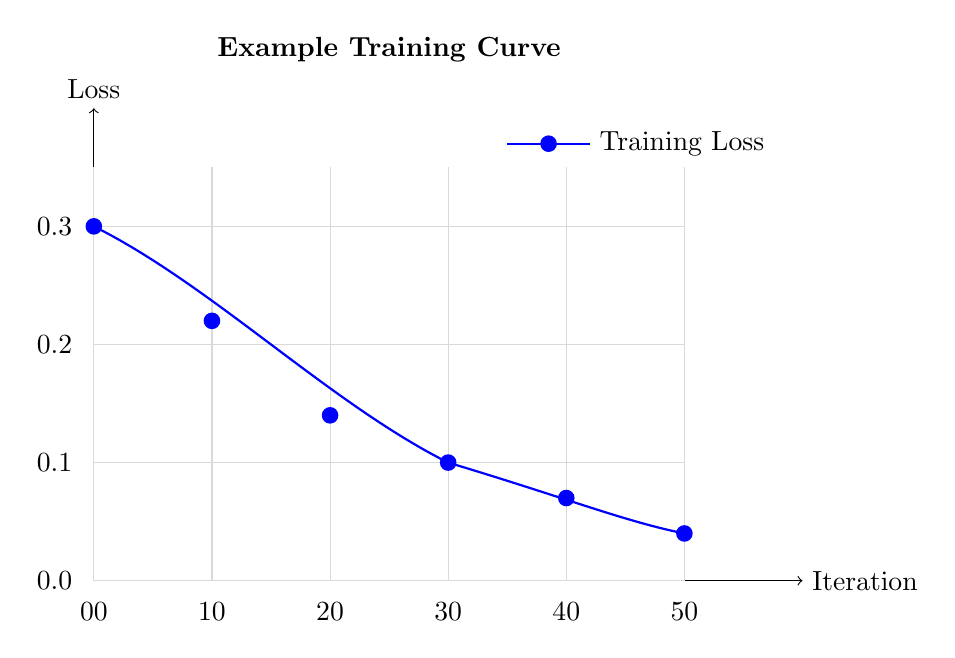
\begin{tikzpicture}[scale=1.5]
  % Draw axes
  \draw[->] (0,0) -- (6,0) node[right] {Iteration};
  \draw[->] (0,0) -- (0,4) node[above] {Loss};

  % Draw grid
  \draw[gray!30] (0,0) grid[step=1] (5,3.5);

  % Draw title
  \node at (2.5, 4.5) {\textbf{Example Training Curve}};

  % Draw training curve (simple exponential decay)
  \draw[blue, thick]
    (0,3) .. controls (1,2.5) and (2,1.5) .. (3,1)
    .. controls (4,0.7) and (4.5,0.5) .. (5,0.4);

  % Add some data points
  \foreach \x/\y in {0/3, 1/2.2, 2/1.4, 3/1, 4/0.7, 5/0.4} {
    \fill[blue] (\x,\y) circle (2pt);
  }

  % Legend
  \draw[blue, thick] (3.5,3.7) -- (4.2,3.7);
  \fill[blue] (3.85,3.7) circle (2pt);
  \node[right] at (4.2,3.7) {Training Loss};

  % Axis labels
  \foreach \x in {0,1,2,3,4,5} {
    \node[below] at (\x,-0.1) {\x 0};
  }
  \foreach \y in {0,1,2,3} {
    \node[left] at (-0.1,\y) {0.\y};
  }
\end{tikzpicture}
\end{document}
